\documentclass[12pt]{article}
\usepackage[english]{babel}
\usepackage{csquotes}
\usepackage{amsmath}
\usepackage{amssymb}
\usepackage{parskip}
\usepackage{verbatim}
\usepackage{authblk}
\usepackage[svgnames]{xcolor}
\usepackage{listings}
\usepackage{hyperref}
\usepackage{fancyvrb}
\usepackage{multirow}
\usepackage{graphicx}
\usepackage[style=authoryear,backend=biber,sorting=nyt,natbib=true]{biblatex}
\graphicspath{ {./} }
\usepackage{setspace}
\onehalfspacing
\addbibresource{assignment.bib}
\emergencystretch=1em

\lstset{language=R,
    basicstyle=\footnotesize\ttfamily,
    stringstyle=\color{DarkGreen},
    otherkeywords={0,1,2,3,4,5,6,7,8,9},
    morekeywords={TRUE,FALSE},
    deletekeywords={data,frame,length,as,character},
    keywordstyle=\color{blue},
    commentstyle=\color{DarkGreen},
    columns=fullflexible
} 

\date{July 2024}


\title{\huge Assignment on Multinomial Regression}
\author{\Large Geordan Ramsamy \textbf{2113888}, \\
         Adriana Laurent \textbf{2116470}, \\
         Dhushiven Moothia \textbf{2118330}, \\
         Saraspadee Chinasamy \textbf{2116979}, \\
         Urumi Ayikullu \textbf{2011016}}
\affil{BSc (Hons) Business statistics with finance \\ Year 3}
\affil{University of Mauritius}

\begin{document}

\maketitle
\clearpage
\tableofcontents

\clearpage

\section*{Introduction}
\addcontentsline{toc}{section}{Introduction}

In this assignment, we will explain the multinomial model and show how it is part of the exponential family. Then, assuming a set of regressors we will define the probability of the $i^{th}$ subject of being in category j, $\pi_{ij}$. Following that, we will simulate a dataset in R on which will apply the multinomial regression. This will enable us to validate the theory of the multinomial model. After that, we will interpret the outputs of the model to get an idea about the effect that our explanatory variables have on the response variable.

\section{Question 1}
\textbf{Using appropriate notations, explain the multinomial model and show the multinomial model is part of the exponential dispersion family.}

\subsection{General equation of a distribution that is part of Exponential Family of distributions.}
\begin{equation}
  p(y|\theta) = h(y)\exp \{ \eta(\theta)^\intercal T(y) - A(\eta) \}
\end{equation}
where, 
\begin{equation*}
  A(\eta) = \log \int h(y) \exp \{ \eta(\theta)^\intercal T(y) \} dy
\end{equation*}

\begin{itemize}
    \item $T(y)$ is the sufficient statistic;
    \item $\eta(\theta)$ is the natural parameter;
    \item $h(y)$ is the underlying measure.
\end{itemize}

All distributions that are part of the exponential dispersion family can have their distribution function rearranged into this form. Changing the different parts of the equation like the sufficient statistic, the natural parameter and the underlying measure will lead to different distributions. The mulitinomial distribution is part of the exponential dispersion family and this will be shown in the next section.

\subsection{Proof}
Let
\begin{enumerate}
    \item $Y_i$ be a random variable $i=1,2,\dots,k$
    \item $n \in \mathbb{N}$ be the number of trials.
    \item $y_{i}\in \mathbb{N}$ be the i-th events in a sequence of n trials.
    \item $\pi_i \in [0,1]$ be the probability of the i-th event of each trial.
\end{enumerate}

The multinomial distribution has the following probability mass function:
\begin{eqnarray*}
  f(y) ~=~ f(y_1, \dots, y_m)
       & = & \text{P}(Y_1 = y_1, \dots, Y_m = y_k) \\
       & = & \frac{n!}{y_1! \cdots y_k!} \prod_{i = 1}^k \pi_i^{y_i}.
\end{eqnarray*}

Where \( \sum_{i=1}^k y_i = n\) and \( \sum_{i=1}^k \pi_i = 1\).

\[
    P(y|\pi) = \exp\left \{ \log \left( \frac{n!}{y_1! y_2! \ldots y_k!} \pi_1^{y_1} \dots \pi_k^{y_k} \right) \right \}
\]
Using law of logarithms:
\begin{eqnarray*}
P(y|\pi) &=& \frac{n!}{y_1! y_2! \ldots y_k!} \exp \left \{ \sum_{i=1}^k \log \pi_i^{y_i} \right \} \\
         &=& \frac{n!}{y_1! y_2! \ldots y_k!} \exp \left \{ \sum_{i=1}^k y_i \log \pi_i \right \}
\end{eqnarray*}

To put this in exponential family form, we eliminate \(\pi_k\) and the corresponding component of \(y\) to keep the same dimensionality:
\begin{eqnarray*}
    P(y|\pi) &=& \frac{n!}{y_1! y_2! \ldots y_{k}!} \exp \left \{ \sum_{i=1}^{k-1} y_i \log \pi_i + \left(n - \sum_{i=1}^{k-1} y_i\right) \log \left(1 - \sum_{i=1}^{k-1} \pi_i \right) \right \} \\
            &=& \frac{n!}{y_1! y_2! \ldots y_{k}!} \exp \left \{ \sum_{i=1}^{k-1} y_i \log  \frac{\pi_i}{1 - \sum_{i=1}^{k-1} \pi_i} + n\log \left(1 - \sum_{i=1}^{k-1} \pi_i \right) \right \}
\end{eqnarray*}

\begin{equation}
    \begin{split}
              P(y|\pi)  = \frac{n!}{y_1! y_2! \ldots y_{k}!} \exp \biggl \{   \begin{bmatrix} \log \frac{\pi_1}{1 - \sum_{i=1}^{k-1} \pi_i} \dots \log  \frac{\pi_{k-1}}{1 - \sum_{i=1}^{k-1} \pi_i} \end{bmatrix} \begin{bmatrix} y_1 \\ \vdots \\ y_{k-1} \end{bmatrix} \\ - - n\log \left(1 - \sum_{i=1}^{k-1} \pi_i \right) \biggr \}
            \end{split}
\end{equation} 


Now that it is in the correct arrangement, we can find out the different parameters of the exponential family that make up the multinomial distribution.

\[
h(y) = \frac{n!}{y_1! y_2! \ldots y_{k}!}
\]
\[
T(y) = \begin{bmatrix}
    y_1 \\ y_2 \\ \vdots \\ y_{k-1}
\end{bmatrix}
\]
\[
\eta(p) = \begin{bmatrix} 
    \log \frac{\pi_1}{1 - \sum_{i=1}^{k-1} \pi_i} \\ \vdots \\ \log \frac{\pi_{k-1}}{1 - \sum_{i=1}^{k-1} \pi_i}
\end{bmatrix} 
\]
Therefore, 
\[\theta_i = \log \left( \frac{\pi_i}{ 1 - \sum_{i=1}^{k-1} \pi_i } \right) \]

Reintroducing \(\pi_k = 1 - \sum_{i=1}^{k-1} \pi_i \), we have:
\begin{eqnarray*}
    \theta_i &=& \log \left ( \frac{\pi_i}{\pi_k} \right) \\
    e^{\theta_i} &=& \frac{\pi_i}{\pi_k} \\
    \pi_i &=& e^{\theta_i}\pi_k
\end{eqnarray*}
Which holds for \(i = k\), if we define \(\theta_k = 0\), which we can do since we haven't defined what \( \theta_k \) is until now.

Since all \(\pi_i\) sum to 1, we get:
\begin{eqnarray*}
    1 &=& \sum_{i=1}^{k} \pi_k \exp(\theta_i) =  \pi_k \sum_{i=1}^{k} \exp(\theta_i) = \pi_k \sum_{i=1}^{k-1} \exp(\theta_i) + \pi_k \exp{(0)} \\
    &=& \pi_k \left( 1 + \sum_{i=1}^{k-1} \exp(\theta_i) \right)
\end{eqnarray*}
Thus, 
\[
\pi_k = \frac{1}{1 + \sum_{i=1}^{k-1} \exp(\theta_i)}
\]
\[
\pi_i = \frac{\exp(\theta_i)}{1 + \sum_{i=1}^{k-1} \exp(\theta_i)}
\]

The log-partition function in terms of \(\pi\) is:
\[ A(\pi) = -n \log (1 - \sum_{i=1} ^{k-1} \pi_i)\]

Rewriting it in terms of \(\theta\):
\begin{eqnarray*}
    A(\theta) &=& - n \log \left(1 + \sum_{i=1}^{k-1} \frac{\exp(\theta_i)}{1 + \sum_{i=1}^{k-1} \exp(\theta_i)} \right) \\
              &=& - n \log \left( \frac{1}{1 + \sum_{i=1}^{k-1} \exp(\theta_i)} \right) \\
              &=& n \log \left(1 + \sum_{i=1}^{k-1} \exp(\theta_i)\right)
\end{eqnarray*}

Hence proved.
\section{Question 2}
\textbf{Assuming set of regressors, provide an expression for the probability for the ith subject in the multinomial model.}
\subsection{Multinomial model explanation}


The dependent variables of a multinomial distribution, $y_i$ has m unordered mutually exclusive outcomes. The outcomes are $j= 1, 2,\dots, m$. The aim is to measure the probabilities of possible occurrence of outcomes, given covariates. The covariates can be of two types: 
\begin{enumerate}
    \item  individual specific set of regressors $x_i$
    \item alternative set of regressors $z_{ij}$. 
\end{enumerate}

This can be denoted as:
\begin{equation*}
  \pi_{ij} ~=~ \text{P}(y_i = j ~|~ x_i, z_{ij})
\end{equation*}
where, $\pi_{ij}$ means the probabilities of occurrence of each outcome.

It is to be noted that, m has to be both mutually exclusive and collectively exhaustive and each outcome is obligatorily between 0 and 1: $0 ~\le~ \pi_{ij} ~\le~ 1$. Moreover, probabilities of each category should sum to one: $i = 1, \dots, n$ and we can have m-1 maximum coefficients to compare probability of a category to a base category.

To begin, we consider N independently identically distributed experiments, leading to one of m mutually exclusive outcomes:  $A_1, \dots, A_m$.

Assuming $Y_l = (Y_{1l}, \dots, Y_{ml})$,

The vector valued indicators will be as follows:
\begin{equation*}
Y_{jl} =
    \begin{cases}
  1 & \text{if $A_j$ is observed in $l$-th experiment,} \\
  0 & \text{otherwise.}
    \end{cases}
\end{equation*}
where $\sum_{j = 1}^m Y_{jl} = 1$.  $Y_{jl}$ and  $Y_{kl}$ are dependent.

Let $X = (X_1, \dots, X_m)$, where, $X_j = \sum_{l = 1}^N Y_{jl}$.

This represents the number of observations of $A_j$ in N trials. It is also to be noted that, $\sum_{j = 1}^m X_j = N$. When variable X is multinomially distributed with N number of trials and with m possible outcomes with their corresponding occurrence probabilities, it is denoted as follows:
$$ X \sim \mathit{MN}(N, \pi_1, \dots, \pi_m) $$

It is to be highlighted that, the probability density function for $x_j \in \{0, 1, \dots, N\}$ and $\sum_{j = 1}^m x_j = N$ is

\begin{eqnarray*}
  f(x) ~=~ f(x_1, \dots, x_m)
       & = & \text{P}(X_1 = x_1, \dots, X_m = x_m) \\
       & = & \frac{N!}{x_1! \cdots x_m!} \prod_{j = 1}^m \pi_j^{x_j}.
\end{eqnarray*}

\subsection{Multinomial logit model}
Coming to the multinomial logit model, it is considered to be the simplest among the multinomial response model. When $Y_i$, that is the response variable has i independent observations, where, $i = 1, \dots, n$ observations, it is expressed as follows:
$$Y_i \sim \mathit{MN}(1, \pi_{i1}, \dots, \pi_{im})$$

We consider only the individual specific set of regressors, $x_i$ as covariates.
Then, the outcome is denoted as: $$y_i \in \{1, \dots, m\}$$ for each $i = 1, \dots, n$ and the corresponding binary indicators denoted by: 
$$d_{ij} \in \{0, 1\}$$

for each $j = 1, \dots, m$ category.
\begin{equation*}
  d_{ij} ~=~  \begin{cases}
             1 & \text{if $y_i = j$,}\\
         0 & \text{otherwise.}
             \end{cases}
\end{equation*}
The joint distribution of the multinomial probability function is:
\begin{equation*}
  f(y_i ~|~ x_i) ~=~ \pi_{i1}^{d_{i1}} \cdots \pi_{im}^{d_{im}} ~=~ \prod_{j = 1}^m \pi_{ij}^{d_{ij}},
\end{equation*}

with $\sum_{j = 1}^m \pi_{ij} = 1$ and $\sum_{j = 1}^m d_{ij} = 1$ for $i = 1, \dots, n$, due to the constraint that the probability of all outcomes sum up to one. Without losing generality, it is then denoted as:
\begin{equation*}
  \pi_{i1} ~=~ 1 ~-~ \sum_{j = 2}^m \pi_{ij}
\end{equation*}

\subsection{Multinomial logit link}
To link the regressors  $x_i$ with the parameters $\pi_{i}$, we use a linear predictor $\eta_{ij}$ based on alternative-specific coefficients  $\beta_{j}$. Then, we link the linear predictor to log-odds. For a multinomial model, the log-odds are the success probability of category j compared to success probability of category 1. In other words, it is the success probability with respect to a reference category.

\begin{equation}
    \label{eqn:logodds}
  \log \left( \frac{\pi_{ij}}{\pi_{i1}} \right) ~=~ \eta_{ij} ~=~ x_i^\top \beta_j, \qquad (j = 2, \dots, m)
\end{equation}

Further elaboration leads to the following:
\begin{eqnarray*}
  \pi_{ij} & = & \exp(\eta_{ij}) \cdot \pi_{i1} \qquad (j = 2, \dots, m), \\
  \pi_{i1} & = & 1 - \pi_{i1} \sum_{s = 2}^m \exp(\eta_{is})
\end{eqnarray*}
This is equivalent to:
\begin{eqnarray*}
\pi_{ij} & = & \frac{\exp(x_i^\top \beta_j)}{1 + \sum_{s = 2}^m \exp(x_i^\top \beta_s)} \qquad (j = 2, \dots, m), \\
  \pi_{i1} & = & \ 1 - \pi_{i1} \sum_{s = 2}^m \exp(x_i^\top \beta_s)  \\
1 & = & \pi_{i1} +  \pi_{i1} \sum_{s = 2}^m \exp(x_i^\top \beta_s)  \\ 
1 & = & \pi_{i1} \cdot \{1 + \sum_{s = 2}^m
 \exp(x_i^\top \beta_s)\}\\ 
\end{eqnarray*}

This indeed leads to the following result:
\begin{equation}
      \pi_{i1} = \frac{1}{1 + \sum_{s = 2}^m \exp(x_i^\top \beta_s)}
\end{equation}

More compactly, we can also write the Multinomial Logit Model as follows:
\begin{equation}
  \pi_{ij} ~=~ \frac{\exp(x_i^\top \beta_j)}{\sum_{s = 1}^m \exp(x_i^\top \beta_s)},
\end{equation}

where, $j = 1, \dots, m$ and $\beta_1 = 0$ is used as identification restriction which results into making category 1 to be termed as the reference category.

It is important to note that the reference category is arbitrarily chosen and that, any other $ \beta_j $ can also be used as the reference category. The Multinomial Model is a multiple index model for m $>$ 2.

\section{Question 3}
\textbf{Create a toy example (or a simulation study) of the multinomial regression model, specifying the input parameters and run the multinomial
regression model using R. Interpret your outputs. [Hint: You may refer to libraries in R for implementing the multinomial regression model]}

\subsection{Dataset Description}
To create a toy example of a multinomial regression model, we created synthetic enrollment data for a university, detailing the socioeconomic status of students (ses), their writing score at the entrance exam (write) and the school type they attended before university (schtyp). The goal of our modelling is to find out how this information affects the program type that they get into (prog). 

\begin{enumerate}
    \item "ses" is a categorical variable with three levels, low, middle and high.
    \item "write" has a normal distribution for low socioeconomic status and skewed-normal for middle and high socioeconomic status, around different means and sds.
    \item "schtyp" is also a categorical variable with two levels, public and private, with different proportions of students going to public or private schools based on their socioeconomic status.
    \item "prog", the target variable, is categorical with three levels academy, general and vocation with academy being the reference category.
\end{enumerate}

After generating the dataset, with 10,000 students so as to minimize the standard error on the estimates, we defined the two linear predictors for general and vocation programs. Then we created a matrix of probabilities using the linear predictors and the formula for $\pi_i$. Using the generated probabilities, the vector for program type is created. Now that the dataset has been generated, we can use the multinom function from the package nnet to fit the multinomial regression model on the data.

\subsection{Linear predictors}
Referring to the equation on the log odds (\ref{eqn:logodds}), and expanding it we get linear predictors:
\[\log(\pi_j/\pi_1) = \beta_{j0} + \beta_{j1}x_{1} + \beta_{j2}x_2 + \beta_{j3}x_{3}\]

\begin{eqnarray*}
\text{lp general} = 2.39 + -0.43 \cdot x_{12} + -1.10 \cdot x_{13} + -0.06 \cdot x_2 + 0.48 \cdot x_{32} \\
\text{lp vocation} = 3.23 + 0.51 \cdot x_{12} + -0.83 \cdot x_{13} + -0.11 \cdot x_{2} + 1.84 \cdot x_{32}
\end{eqnarray*}

\subsection{Coefficients Explanation}
Here are the model coefficients and standard errors.
\begin{Verbatim}[fontsize=\small]
Call:
multinom(formula = prog ~ ses + write + schtyp, data = enrollment, 
    trace = FALSE)

Coefficients:
         (Intercept)  sesmiddle   seshigh       write schtyppublic
general     2.274338 -0.4205934 -1.063186 -0.05631971    0.3770877
vocation    3.169315  0.4141368 -1.022549 -0.10310304    1.6454736

Std. Errors:
         (Intercept)  sesmiddle    seshigh      write schtyppublic
general    0.1750069 0.06590892 0.07458548 0.00306963   0.07268874
vocation   0.1828433 0.06697754 0.08454983 0.00322049   0.09500439

Residual Deviance: 17670.02 
AIC: 17690.02 
\end{Verbatim}

We got back the coefficients that we used in our linear predictors, within a margin of error, thereby verifying the theory of the previous sections. 

As expected, the standard error on the estimates are quite low. However, the model has a high deviance of 17670 and Akaike Information Criterion (AIC) of 17690 which could mean that the model is not a good fit for the data. We can compare these values with a model that is fit only on the intercept to see if our variables improved the model or not. 

\begin{Verbatim}[fontsize=\small]
summary(multinom(prog ~ 1, data = enrollment))
# weights:  6 (2 variable)
initial  value 10986.122887 
final  value 10085.209388 
converged
Call:
multinom(formula = prog ~ 1, data = enrollment)

Coefficients:
         (Intercept)
general   -0.9404609
vocation  -0.7594095

Std. Errors:
         (Intercept)
general   0.02572553
vocation  0.02414497

Residual Deviance: 20170.42 
AIC: 20174.42 
\end{Verbatim}

This shows that our variables explain the data better than just the intercept. We also checked if the variables themselves are all significant in the model by computing an Anova of the model. If the p value for each variable is $<0.05$, we know that the variable has an effect on the model. 
\begin{Verbatim}[fontsize=\small] 
car::Anova(m)
Analysis of Deviance Table (Type II tests)

Response: prog
       LR Chisq Df Pr(>Chisq)    
ses      590.59  4  < 2.2e-16 ***
write   1264.58  2  < 2.2e-16 ***
schtyp   378.95  2  < 2.2e-16 ***
---
\end{Verbatim}

All 3 variables are thus signficant at the 95\% level. 

Exponentiating the coefficients gives the relative risk ratio (RRR) of variable with respect to the base category.

\begin{Verbatim}[fontsize=\small]
exp(coef(m))
         (Intercept) sesmiddle   seshigh     write schtyppublic
general     9.721479 0.6566571 0.3453539 0.9452369     1.458032
vocation   23.791172 1.5130641 0.3596769 0.9020340     5.183464
\end{Verbatim}

For example, the RRR of sesmiddle for general is 0.66. This means that students from a middle socioeconomic status compared are 0.66 times as likely to be in the general program compared to academy as one with a low socioeconomic status. In other words, the odds of being in general decreased by 34\% compared to academy. The RRR of write for vocation is 0.90. This means that for each unit increase in writing scores, the odds of being in vocation compared to academy decreased by 10\%. Finally, the RRR schtyppublic for vocation is 5.18. This means that students that went to a public school were 5.18 times as likely as students who went to private school to be in the vocation program compared to the academy program. 

\clearpage
\subsection{Effects plots}

We can also visualize the effect that each variable had on the probability of being in each program type.

\begin{figure}[h]
\centering
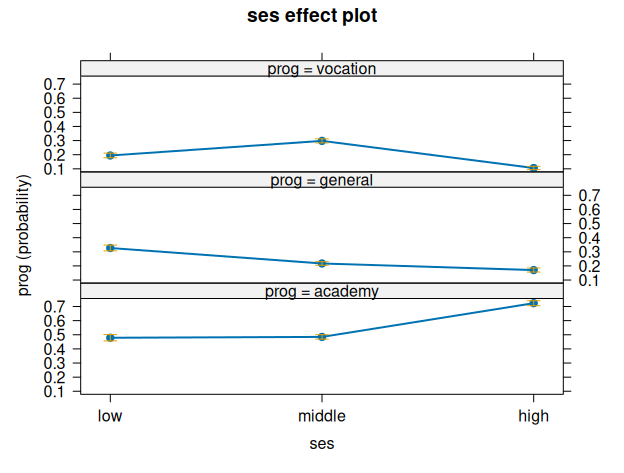
\includegraphics[scale=0.7]{Rplot01.png}
\caption{ses effects}
\end{figure}


As shown in Figure 1, when ses was high the probability of being in academy was much higher than the probability of being in other programs.
 \clearpage
\begin{figure}[h]
\centering
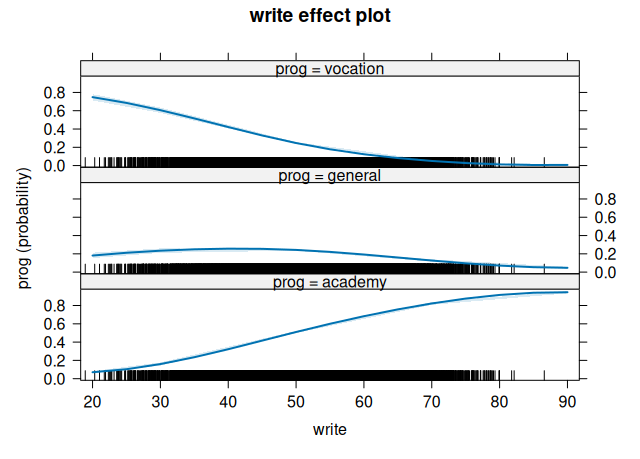
\includegraphics[scale=0.7]{Rplot02.png}
\caption{write effects}
\end{figure}


Figure 2 describes how a higher writing score leads to a steady decrease in the probability of being in programs other than academy.
\clearpage 

\begin{figure}[ht]
\centering
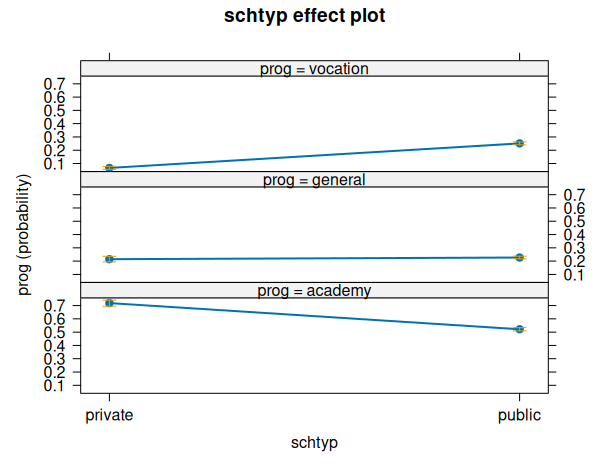
\includegraphics[scale=0.7]{Rplot03.png}
\caption{schtyp effects}
\end{figure}

From Figure 3 we see that, while being from a public school decreased the probability of being in academy, it was still at 0.6, showing that the model favoured academy a lot more than other program types. 

\clearpage

\subsection{Confusion matrix}

We can draw a confusion matrix to show this imbalance.
\begin{verbatim}
pred_acc <- table(enrollment$prog, predict(m, enrollment[2:4]))
pred_acc
\end{verbatim}

\begin{table}[h]
\centering
\begin{tabular}{|c|l|lll|}
\hline
\multicolumn{1}{|l|}{}           &          & \multicolumn{3}{c|}{\textbf{Predicted}}                                \\ \hline
\multicolumn{1}{|l|}{}           &          & \multicolumn{1}{l|}{academy} & \multicolumn{1}{l|}{general} & vocation \\ \hline
\multirow{3}{*}{\textbf{Actual}} & academy  & \multicolumn{1}{l|}{4730}    & \multicolumn{1}{l|}{23}      & 628      \\ \cline{2-5} 
                                 & general  & \multicolumn{1}{l|}{1459}    & \multicolumn{1}{l|}{31}      & 611      \\ \cline{2-5} 
                                 & vocation & \multicolumn{1}{l|}{1237}    & \multicolumn{1}{l|}{30}      & 1251     \\ \hline
\end{tabular}
\caption{Confusion Matrix}
\end{table}
Table 1 shows the confusion matrix of our model predictions. We see that especially for general program types, a lot were misclassified as academy. The same can be found for vocation even if it has a better prediction accuracy than general. Academy was the most correctly classified outcome.

\section*{Conclusion}
\addcontentsline{toc}{section}{Conclusion}
In this assignment, we applied the Multinomial Regression model using a toy dataset to show its functionality and interpret the outcomes. The synthetic data helped to demonstrate how different variables can theoretically impact categorical outcomes, such as enrollment probabilities in educational programs. We highlighted the model's coefficients and standard errors, emphasizing its robustness while also pointing out the model's shortcomings.

\section*{Citations}
\addcontentsline{toc}{section}{Citations}
A lot of the proof for question 1 derives from \cite{geyer_stat_nodate}, \cite{statisticsmatt_exponential_2019} and
\cite{stackex}. For question 2, it is mainly inspired from \cite{discdown}. The original dataset used to estimate coefficients and data distributions for the synthetic data comes from \cite{multinomial_example}. The simulation itself is done with the help of \cite{simulation_article} from which the code structure comes from. Last mention is the wikipedia articles \cite{wikipedia_multinomial} and \cite{wikipedia_exponential} which have helped when trying to understand the subject.

\section*{Codes}
\addcontentsline{toc}{section}{Codes}
All the code can be found at \url{https://github.com/G3ordan1/multinomial_logit} in the file simulation.R.

\addcontentsline{toc}{section}{References}
\printbibliography

\section*{Annex}
\addcontentsline{toc}{section}{Annex}
\begin{lstlisting}
# Enrollment data for a university detailing the program type 
# of students and some information about them.
# Dependent variable program type. General Academy Vocational
# Predictors: ses (socioeconomic status), write 
# (writing score), schtyp (school type they attended)

# loading required libraries
library(dplyr)
library(nnet)
set.seed(7) # set seed for reproducibility
# Generate a random sample of socioeconomic statuses (ses)
ses <- sample( 
  c("low", "middle", "high"),  # Categories to sample from
  size = 10000L,               # Sample size of 10,000
  replace = TRUE,              # Allow repetition in sampling
  prob = c(0.235, 0.475, 0.29) 
  # Probability weights for each category
)


# Convert the 'ses' vector to a factor with specified levels
ses <- factor(ses, levels = c("low", "middle", "high"))

# Define parameters for skew-normal distribution for write 
# with "high" SES
high_params <- sn::cp2dp(c(56, 9.44, -0.5), "SN")

# Define mean and standard deviation for normal distribution 
# for write with "low" SES
low_params <- list("mean" = 50.6, "sd" = 9.49)

# Define parameters for skew-normal distribution for write 
# with "middle" SES
middle_params <- sn::cp2dp(c(51.9, 9.11, -0.25), "SN")


# Create a numeric vector of length 10,000 to store data
write <- vector("numeric", 10000L)

# Fill the vector with normally distributed data for "low"
# SES
write[ses == "low"] <- rnorm(sum(ses == "low"), 
                             low_params$mean,
                             low_params$sd)

# Fill the vector with skew-normal distributed data for "middle" SES
write[ses == "middle"] <- sn::rsn(sum(ses == "middle"), 
dp = middle_params)

# Fill the vector with skew-normal distributed data for "high" SES
write[ses == "high"] <- sn::rsn(sum(ses == "high"), dp = high_params)

# Create a character vector of length 10,000 to store school types
schtyp <- vector("character", 10000L)

# Assign school types to subjects with "low" SES with specified 
# probabilities
schtyp[ses == "low"] <- sample(c("private", "public"), sum(ses == "low"),
                                replace = TRUE, prob = c(0.04, 0.96))

# Assign school types to subjects with "middle" SES with specified 
# probabilities
schtyp[ses == "middle"] <- sample(c("private", "public"), 
                                    sum(ses == "middle"),
                                    replace = TRUE,
                                    prob = c(0.2, 0.8))

# Assign school types to subjects with "high" SES with specified 
probabilities
schtyp[ses == "high"] <- sample(c("private", "public"),
                                sum(ses == "high"),
                                replace = TRUE,
                                prob = c(0.2, 0.8))

# Calculate the linear predictor for general education
lp_general <- 2.39 + -0.43 * (ses == "middle") + -1.10 * (ses == "high") +
-0.06 * write + 0.48 * (schtyp == "public")

# Calculate the linear predictor for vocational education
lp_vocation <- 3.23 + 0.51 * (ses == "middle") + -0.83 * (ses == "high") +
-0.11 * write + 1.84 * (schtyp == "public")

# Calculate the denominator for the multinomial logistic 
# model probabilities
denominator <- (1 + exp(lp_general) + exp(lp_vocation))

# Calculate the probability of the first outcome
p1 <- 1 / denominator

# Calculate the probability of the second outcome (general education)
p2 <- exp(lp_general) / denominator

# Calculate the probability of the third outcome (vocational education)
p3 <- exp(lp_vocation) / denominator

# Combine the probabilities into a matrix
P <- cbind(p1, p2, p3)

# Display the first few rows of the probability matrix
head(P)

# Check that the sum of probabilities for each row is 1
all(round(apply(P, 1, sum)) == 1)

# Simulate enrollment outcomes based on the probabilities
y <- apply(P, MARGIN = 1,
            function(x) sample(x = c("academy", "general", "vocation"),
                                size = 1, prob = x)
                                )

# Convert the outcome variable to a factor with specified levels
y <- factor(y, levels = c("academy", "general", "vocation"))

# Display the frequency table of the outcome variable
table(y)

# Create a data frame with the simulated data
enrollment <- data.frame(prog = y, write, ses, schtyp)

# Display the structure of the data frame
str(enrollment)

# Fit a multinomial logistic regression model
m <- multinom(prog ~ ses + write + schtyp,
                data = enrollment,
                trace = FALSE)

# Display a summary of the model
summary(m)

# RRR
exp(coef(m))

# Perform an ANOVA on the model
car::Anova(m)

# Fit on intercept
summary(multinom(prog ~ 1, data = enrollment))

# Plot how the variables affect the probability of being in a category
library(effects)
effects <- allEffects(m)
plot(effects$ses)
plot(effects$write)
plot(effects$schtyp)

# Confusion matrix
pred_acc <- table(enrollment$prog, predict(m, enrollment[2:4]))
pred_acc

\end{lstlisting}
\end{document}


